\documentclass[hidelinks, 12pt]{article}
\usepackage[italian]{babel}
\usepackage{natbib}
\usepackage{url}
\usepackage[utf8x]{inputenc}
\usepackage{amsmath}
\usepackage{graphicx}
\graphicspath{{images/}}
\usepackage{parskip}
\usepackage{fancyhdr}
\usepackage{vmargin}
\usepackage{float}
\usepackage{hyperref}
\usepackage{subfig}
\setmarginsrb{3 cm}{2.5 cm}{3 cm}{2.5 cm}{1 cm}{1.5 cm}{1 cm}{1.5 cm}

\title{Amazon Reviews Sentiment Analysis}				% Title
\author{Basso Matteo \\ Ferri Marco}								% Author
\date{Luglio 2019}				% Date

\makeatletter
\let\thetitle\@title
\let\theauthor\@author
\let\thedate\@date
\makeatother

\pagestyle{fancy}
\fancyhf{}
\rhead{Basso M., Ferri M.}
\lhead{\thetitle}
\cfoot{\thepage}

\begin{document}
	
%%%%%%%%%%%%%%%%%%%%%%%%%%%%%%%%%%%%%%%%%%%%%%%%%%%%%%%%%%%%%%%%%%%%%%%%%%%%%%%%%%%%%%%%%

\begin{titlepage}
	\centering
	\vspace*{0.5 cm}
	
\includegraphics[scale = 0.75]{images/LogoBicocca.pdf}\\[1.0 cm]	% University Logo
	\textsc{\LARGE Università degli studi di}\\[0.2 cm]
	\textsc{\LARGE Milano-Bicocca}\\[2.0 cm]	% University Name
	\textsc{\Large F1801Q104}\\[0.5 cm]				% Course Code
	\textsc{\large Data Analytics}				% Course Name
	\rule{\linewidth}{0.2 mm} \\[0.4 cm]
	{ \huge \bfseries \thetitle}\\
	\rule{\linewidth}{0.2 mm} \\[1.5 cm]
	
	\begin{minipage}{0.4\textwidth}
		\begin{flushleft} \large
			\emph{Studenti:}\\
			\theauthor
		\end{flushleft}
	\end{minipage}~
	\begin{minipage}{0.4\textwidth}
		\begin{flushright} \large
			\emph{Matricole:} \\
			807628 \\ 807130
		\end{flushright}
	\end{minipage}\\[2 cm]
	
	{\large \thedate}\\[2 cm]
	
	\vfill
	
\end{titlepage}

%%%%%%%%%%%%%%%%%%%%%%%%%%%%%%%%%%%%%%%%%%%%%%%%%%%%%%%%%%%%%%%%%%%%%%%%%%%%%%%%%%%%%%%%%


\null\vspace{\stretch{1}}
\section*{\centering Abstract}

Lorem ipsum dolor sit amet.

\vspace{\stretch{2}} \null

\clearpage


%%%%%%%%%%%%%%%%%%%%%%%%%%%%%%%%%%%%%%%%%%%%%%%%%%%%%%%%%%%%%%%%%%%%%%%%%%%%%%%%%%%%%%%%%

\tableofcontents
\clearpage
\listoffigures
\listoftables
\pagebreak

%%%%%%%%%%%%%%%%%%%%%%%%%%%%%%%%%%%%%%%%%%%%%%%%%%%%%%%%%%%%%%%%%%%%%%%%%%%%%%%%%%%%%%%%%



\section{Introduzione}


Lo studio ha lo scopo di condurre diversi tipi di analisi sulle recensioni del noto portale e-commerce Amazon \cite{site:amazon}. In questa sezione viene presentata una breve introduzione al problema, il dataset utilizzato e gli strumenti che sono stati impiegati per portare a termini gli obiettivi prefissati.



\subsection{Dominio di riferimento}

Sempre maggiore è il numero di siti web che fanno delle recensioni il proprio principale business. Si pensi ai portali dedicati alla recensione di località turistiche, film o ristoranti. Allo stesso modo, anche Amazon basa sulle recensioni parte della propria fidelizzazione clienti.

Trattandosi di dati testuali prodotti dagli utenti per valutare i prodotti acquistati, le recensioni esprimono attraverso il linguaggio naturale le impressioni dell'autore, le quali possono assumere un carattere di natura positiva o negativa. In questo contesto è inoltre pratica comune associare al proprio pensiero un punteggio che esprima una valutazione del prodotto su una scala numerica. Se questa informazione è fondamentale per i clienti della piattaforma, poiché permette di capire a colpo d'occhio quale possa essere la qualità dell'articolo che si sta considerando di acquistare, è anche vero che tale punteggio possa rappresentare un aiuto importante per riassumere in forma strutturata (e pertanto più facilmente comprensibile da un computer) l'opinione dell'autore riguardo un certo argomento. Pertanto, analizzare congiuntamente il testo di una recensione ed il punteggio ad essa associato è fondamentale per determinare una correlazione fra il linguaggio naturale e l'opinione dell'utente nei confronti del prodotto, anche detta \textbf{sentiment}. Inoltre, l'elaborazione del testo può considerare il piano morfologico del linguaggio per derivare l'opinione espressa riguardo le diverse caratteristiche del prodotto, dette \textbf{aspect}, espresse nella recensione. Ciò è particolarmente utile per migliorare la qualità dei propri prodotti e ottenere quindi un vantaggio sul piano commerciale.

Infine, l'analisi delle recensioni può essere utile anche per ottenere un'approssimativa profilazione di un utente; questa può rivelarsi particolarmente rilevante dal punto di vista del marketing, ad esempio per dare suggerimenti ad altri utenti che dimostrano di avere le medesime preferenze. Allo stesso modo, può essere costruito un sistema di suggerimenti basato su prodotti simili o solitamente venduti insieme. Tali tecniche vengono dette di \textbf{collaborative filtering}.

Il seguente elaborato si pone l'obiettivo di sperimentare con i concetti appena presentati per determinare quanto sia possibile ottenere attraverso l'analisi delle recensioni di un portale e-commerce come Amazon.



\subsection{Dataset}
\label{sec:dataset}

Il dataset utilizzato per effettuare le analisi è fornito ufficialmente da Amazon e contiene recensioni redatte in lingua inglese fra il 1996 e il 2014, per diverse categorie di prodotti \cite{site:amazon-reviews-original-dataset}. Poiché contenente un gran numero di recensioni che coinvolgono altrettanti utenti e prodotti, talvolta poco partecipativi all'interno del portale e-commerce, si è scelto di utilizzare ai fini del progetto una versione rielaborata del suddetto dataset, reperibile qui: \url{http://jmcauley.ucsd.edu/data/amazon}. Julian McAuley \cite{site:julianmcauley}, professore dell'Università di San Diego, ha estrapolato dal dataset originale solamente i record delle recensioni riguardanti prodotti e utenti con almeno cinque recensioni ciascuno; ciò viene definito in teoria dei grafi con il termine \textbf{k-core}, cioè un sottografo in cui tutti i nodi hanno un grado almeno pari a \texttt{k} \cite{site:wiki-kcore}.

\nocite{site:amazon-reviews-5-core-dataset}



\subsection{Strumenti}

Per effettuare le analisi mostrate in questo elaborato si è utilizzato prevalentemente il linguaggio di programmazione open source Python, attraverso l'utilizzo di Google Colab \cite{site:google-colab} per la creazione di Jupyter Notebook interattivi. Le specifiche librerie di volta in volta utilizzate saranno presentate contestualmente alle singole analisi qualora lo si ritenesse necessario ai fini di una migliore comprensione del problema.

Per l'analisi della rete di prodotti e utenti ricavata dal dataset si è utilizzato il software Cytoscape \cite{site:cytoscape}, dedicato appositamente all'integrazione e visualizzazione di grafi anche molto complessi. Nell'ultima parte del documento verrà infine presentata una demo Web-based per testare con mano le potenzialità dei concetti studiati.



\clearpage



\section{Basic Analysis}


Il dataset è stato reperito in formato JSON e successivamente letto attraverso Python per la memorizzazione in una struttura adatta ad essere elaborata efficientemente dal linguaggio. A tal fine si è scelto di utilizzare la liberia \texttt{pandas} \cite{site:pandas}, dedicata all'analisi di dati anche molto voluminosi. É interessante notare come la lettura del dataset, ed in particolare la conversione di quest'ultimo dal formato JSON, sia stata una delle operazioni computativamente più \textit{time-consuming} fra tutte quelle effettuate, a dimostrazione del fatto che \texttt{pandas} sia successivamente in grado di elaborare molto velocemente le informazioni memorizzate all'interno dei cosiddetti \texttt{DataFrame}.



\subsection{Schema}

Il dataset può essere descritto molto velocemente, poiché rappresentabile attraverso una singola struttura tabellare composta dai campi illustrati in tabella \ref{tab:df-schema}.

\begin{table}[H]
	\caption{Schema originale del dataset}\label{tab:df-schema}
	\centering
	\begin{tabular}{|l|l|l|}
		\hline
		Campo & Descrizione \\
		\hline
		reviewerID & ID utente \\
		reviewerName & Nome utente \\
		asin & ID prodotto \\
		reviewText & Testo della recensione \\
		summary & Titolo della recensione \\
		helpful & Utilità della recensione \\
		overall & Punteggio \\
		reviewTime & Timestamp in formato string \\
		unixReviewTime & Timestamp in formato unix \\
		\hline
	\end{tabular}
\end{table}

Ogni record è la rappresentazione di una singola recensione, svolta da parte di un utente per un certo prodotto nella data indicata. Mentre per quanto riguarda l'utente si è in possesso sia dell'ID che del nome (che non verrà utilizzato), il prodotto è rappresentato nel dataset solamente attraverso un ID (\texttt{asin}); ulteriori dettagli sul prodotto possono essere ricavati contattando il creatore del dataset attraverso un'apposita richiesta, che non è stata effettuata poiché tali informazioni si sono rivelate ininfluenti ai fini del progetto in esame.

Per quanto riguarda i campi relativi alla recensione, è possibile visualizzare sia il titolo che il testo del corpo, oltre al punteggio espresso su una scala numerica da 1 a 5. Poiché ciò rappresenta il sentiment associato alla recensione, questo attributo costituirà anche la variabile target per l'analisi e l'addestramento dei modelli di machine learning.

Il campo \texttt{helpful} presenta un dominio non particolarmente definito e non è stato considerato per l'analisi, mentre per il timestamp si è computato un attributo \texttt{date} di tipo \textit{datetime}; infine, per semplificare il concetto associato ad ogni campo si è scelto di rinominarli. Al termine della trasformazione, il dataset risultante è il seguente:

\begin{table}[H]
	\caption{Schema modificato del dataset}\label{tab:df-schema-new}
	\centering
	\begin{tabular}{|l|l|l|}
		\hline
		Campo & Descrizione \\
		\hline
		userID & ID utente \\
		productID & ID prodotto \\
		text & Testo della recensione \\
		summary & Titolo della recensione \\
		rating & Punteggio \\
		date & Timestamp in formato datetime \\
		\hline
	\end{tabular}
\end{table}



\subsection{Dimensioni}
\label{sec:dimensions}

Dalla fonte citata nell'introduzione, da cui è stato reperito il dataset, è possibile notare che siano presenti varie possibilità di download. Diverse categorie di prodotti sono state testate durante l'intero sviluppo dello studio, ma ai fini di redigere questo elaborato verrà considerato il dataset 5-core chiamato \textit{Clothing, Shoes and Jewelry}, contenente recensioni relative al mercato dei vestiti, delle scarpe e dei gioielli.

Questo contiene un totale di \textbf{278.677 recensioni}, divise fra \textbf{39.387 utenti} e \textbf{23.033 prodotti}. Ciò significa una media di circa 7 recensioni ad utente e 12 recensioni per prodotto. Nel capitolo \ref{sec:network-anal} verrà mostrata se tale media è anche effettivamente rappresentativa del dataset oppure diversi prodotti ed utenti presentano un numero di recensioni sbilanciato.



\subsection{Distribuzione di \texttt{rating}}
\label{sec:rating-distr}

In figura \ref{fig:rating-distr-orig} è possibile osservare la distribuzione del campo \texttt{rating}, che costituisce l'elemento fondamentale su cui costruire un modello supervisionato di sentiment analysis. Come è possibile osservare, questa variabile è fortemente sbilanciata sui valori 4 e 5, motivo che a fronte di alcune considerazioni future porterà il problema ad essere prima binarizzato e successivamente downsampled per ridurre il gap fra la classe positiva e quella negativa.

\begin{figure}[H]
	\centering
	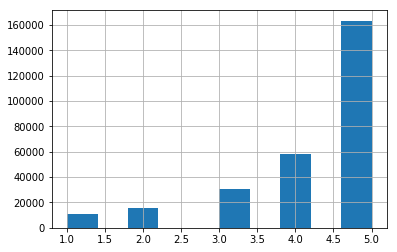
\includegraphics[scale=0.7]{images/02_01_rating_distr.png}
	\caption[Distribuzione del campo \texttt{rating}]{Distribuzione del campo \texttt{rating}}
	\label{fig:rating-distr-orig}
\end{figure}



\subsection{Analisi temporale business-oriented}

Si era già accennato che la fonte fornisca recensioni per più di dieci anni di vendite. Più precisamente, il dataset qui considerato considera recensioni fra il marzo 2003 e giugno 2014 secondo la distribuzione indicata in figura \ref{fig:date-distr}. Pur essendo la maggior parte delle recensioni concentrata negli ultimi 3 anni, qualsiasi sia il filtro temporale applicato non c'è differenza nella distribuzione della variabile target.

\begin{figure}[H]
	\centering
	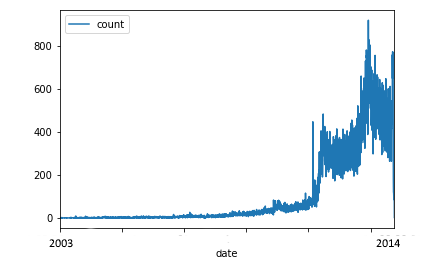
\includegraphics[scale=0.7]{images/02_02_date_distr.png}
	\caption[Distribuzione delle recensioni per data]{Distribuzione delle recensioni per data}
	\label{fig:date-distr}
\end{figure}

\clearpage

Considerato il dominio in esame, potrebbe essere molto utile nell'ottica di prendere decisioni di business per i produttori analizzare come le recensioni si distribuiscono anche in un anno relativamente ai mesi e i giorni della settimana, per evidenziare eventuali periodi di maggiore attività su Amazon. A tal proposito sono pertanto stati prodotti i grafici in figura \ref{fig:month-distr} e \ref{fig:day-distr}.

\begin{figure}[H]
	\centering
	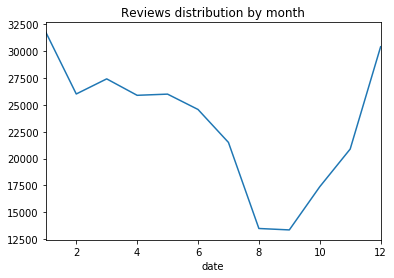
\includegraphics[scale=0.7]{images/02_03_month_distr.png}
	\caption[Distribuzione delle recensioni per mese]{Distribuzione delle recensioni per mese}
	\label{fig:month-distr}
\end{figure}

\begin{figure}[H]
	\centering
	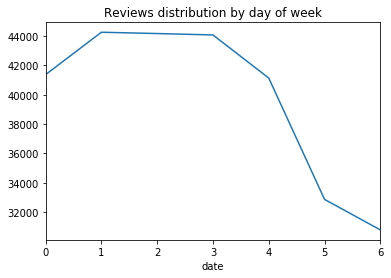
\includegraphics[scale=0.7]{images/02_04_day_distr.png}
	\caption[Distribuzione delle recensioni per giorno della settimana]{Distribuzione delle recensioni per giorno della settimana}
	\label{fig:day-distr}
\end{figure}

Osservando la distribuzione per mese, è possibile notare come la maggiore concentrazione di recensioni si riscontri nel periodo compreso fra il black friday (Novembre) e tutte le vacanze natalizie, probabilmente proprio per via degli sconti e della necessità di comprare regali ai propri conoscenti. É durante questi mesi e quelli immediatamente precedenti che i produttori dovrebbero concentrare maggiormente le proprie campagne pubblicitarie. Tale attività decrementa gradualmente nei mesi successivi a Gennaio, per raggiungere livelli particolarmente bassi ad Agosto e Settembre.

Concentrandoci invece sui dati che riassumono l'andamento di acquisti durante la settimana, è chiaramente evidente come sabato e domenica costituiscano i giorni in cui gli utenti Amazon sono meno propensi a fare recensioni.

Analizzando quindi la distribuzione del \texttt{rating} suddiviso per mesi e giorni, emerge comunque che i risultati sono del tutto analoghi a quelli della figura \ref{fig:rating-distr-orig}. Da questa osservazione si potrebbe concludere che non vi sono particolari periodi temporali durante i quali i clienti sono più propensi a dare recensioni più positive o negative. Ciò su cui le aziende dovrebbero concentrarsi, da questo punto di vista, è solamente la necessità di raggiungere più persone possibili nei momenti di maggiore attività.



\clearpage



\section{Network Analysis}
\label{sec:network-anal}


Nonostante tale elaborato non si concentri sugli aspetti che sia possibile considerare attraverso la rete costituita da utenti, prodotti e recensioni, questo capitolo presenta comunque una breve analisi di tale rete poiché può essere utile ad analizzare il dataset da un punto di vista descrittivo.

\vspace{3ex}

Con un dataset di recensioni è possibile costruire tre diverse tipologie di rete:

\begin{itemize}
	\item prodotti e utenti nella stessa rete, collegati attraverso le recensioni
	\item rete di soli prodotti, collegati tramite similarità
	\item rete di soli utenti, collegati tramite similarità
\end{itemize}

Le due reti che considerano le similarità di prodotti o utenti non sono particolarmente semplici da costruire; esse richiedono che venga definito il concetto stesso di similarità. Ad esempio, prodotti simili potrebbero essere quelli che sono recensiti dai medesimi utenti ed analogamente accade per gli utenti che recensiscono gli stessi prodotti. Questo tipo di relazione potrebbe essere utilizzata per definire delle categorie di utenti o prodotti attraverso algoritmi di \textit{clustering} che andrebbero successivamente interpretati sui metadati contenuti nei nodi, prodotti o utenti che siano. Poiché nel dataset utilizzato mancano questo tipo di informazioni, si è pensato potesse essere poco significativo costruire questi tipi di reti.

Al contrario, ci si è concentrati sulla prima alternativa che è direttamente estraibile dal dataset e consente di carpire se le recensioni coinvolgono omogeneamente diversi prodotti o si suddividono in diverse componenti connesse o cluster.



\subsection{Struttura della rete}

Per generare la rete ci si è affidati alla libreria Python \texttt{NetworkX} \cite{site:networkx}, che consente di generare, modificare e analizzare grafi anche di natura complessa. Per quanto riguarda la parte di visualizzazione si è invece utilizzato il software Cytoscape, che la libreria Python stessa suggerisce per la visualizzazione di reti molto grosse.

La rete è stata generata dal \texttt{pandas DataFrame}, considerando le colonne \texttt{userID} e \texttt{productID} per rappresentare rispettivamente i nodi sorgenti e i nodi target. Ciò significa che si è creata una rete i cui nodi rappresentassero alternativamente utenti o prodotti, nella quale i primi hanno sempre archi diretti verso i secondi: le recensioni. Si è quindi tratto un grafo orientato nel quale i nodi degli utenti hanno solamente archi uscenti e i nodi dei prodotti solo archi entranti. Ciò è particolarmente utile per l'analisi di \textit{in} e \textit{out degree} che si vedrà nella sezione successiva numero \ref{sec:nodes-degree}.

Si è ottenuta quindi una rete composta da \textbf{62.420 nodi} (utenti + prodotti) e \textbf{278.677 archi} (recensioni), quest'ultimi pesati sul \texttt{rating} delle recensioni stesse. Purtroppo una rete così grossa è particolarmente difficile da mostrare correttamente a video anche con Cytoscape, come è possibile notare nell'immagine \ref{fig:cyto-net-1}.

\begin{figure}[H]
	\centering
	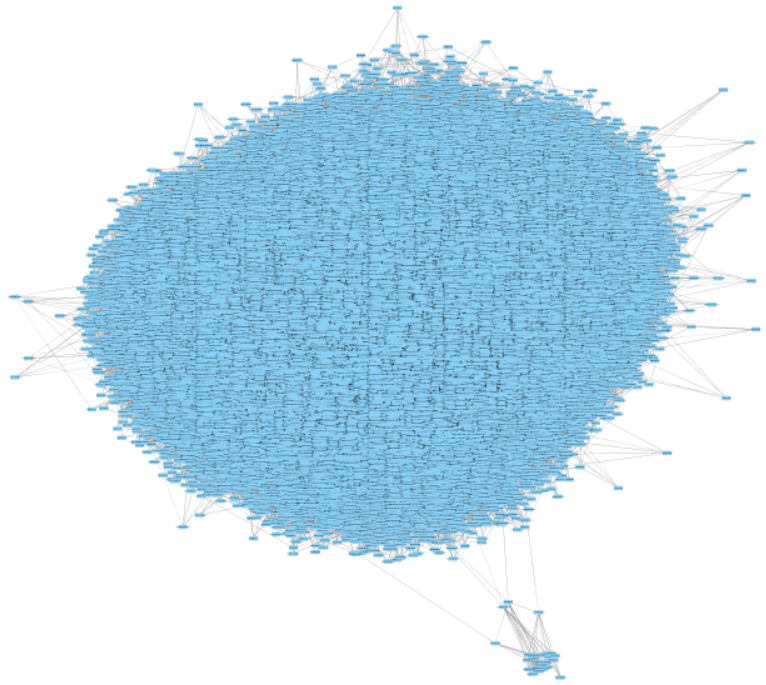
\includegraphics[scale=0.9]{images/03_01_cyto_net_1.png}
	\caption[Rete di utenti e prodotti, collegati tramite recensioni]{Rete di utenti e prodotti, collegati tramite recensioni}
	\label{fig:cyto-net-1}
\end{figure}

É facilmente possibile notare, per quanto sia complessa, che la rete è composta da un'unica grande componente connessa nella quale la maggior parte dei prodotti e degli utenti sono fortemente interconnessi senza apparenti raggruppamenti.

Tuttavia è interessante notare che dall'agglomerato centrale si sviluppano due fenomeni interessanti: alcuni nodi appaiono separati esternamente dal resto del gruppo, come fossero elementi con la voglia di distinguersi dal resto. É il caso ad esempio di quanto accada in figura \ref{fig:cyto-net-2}, che analizza la zona alta destra della rete. Queste due \textit{spike} esterne alla rete sono rispettivamente un prodotto e un utente, come si può notare dalla direzionalità degli archi che li coinvolgono. Purtroppo non è dato sapere se questi vengano posizionati così da Cytoscape perché rappresentano effettivamente dei casi particolari, o solo per una pura casualità.

\begin{figure}[H]
	\centering
	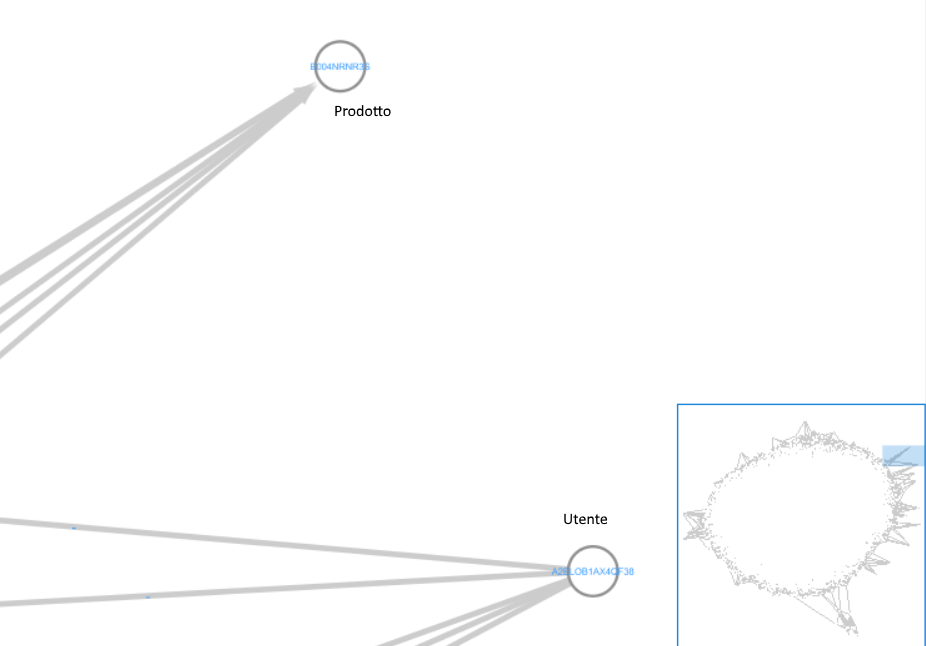
\includegraphics[scale=0.5]{images/03_02_cyto_net_2.png}
	\caption[Esempio di nodi separati dal raggruppamento centrale]{Esempio di nodi separati dal raggruppamento centrale}
	\label{fig:cyto-net-2}
\end{figure}

\vspace{5ex}

Di maggiore interesse appare invece la parte bassa della rete, rappresentata in figura \ref{fig:cyto-net-3}. In questa zona sembra comparire una sorta di cluster vero e proprio, al suo interno fortemente connesso ma collegato alla rete "principale" solo attraverso pochi nodi che svolgono il ruolo di ponte: 3 utenti e 1 prodotto. Nonostante non ci è dato sapere cosa possa rappresentare tale cluster, vista la presenza di alcuni utenti e prodotti con un alto numero di recensioni ma isolati dal resto della rete si potrebbe dedurre si tratti del mercato di un paio d'articoli particolarmente di nicchia, probabilmente provenienti da mercati stranieri o destinati ad un tipo di vendita fra gruppi ristretti di persone con particolari accordi.

\begin{figure}[H]
	\centering
	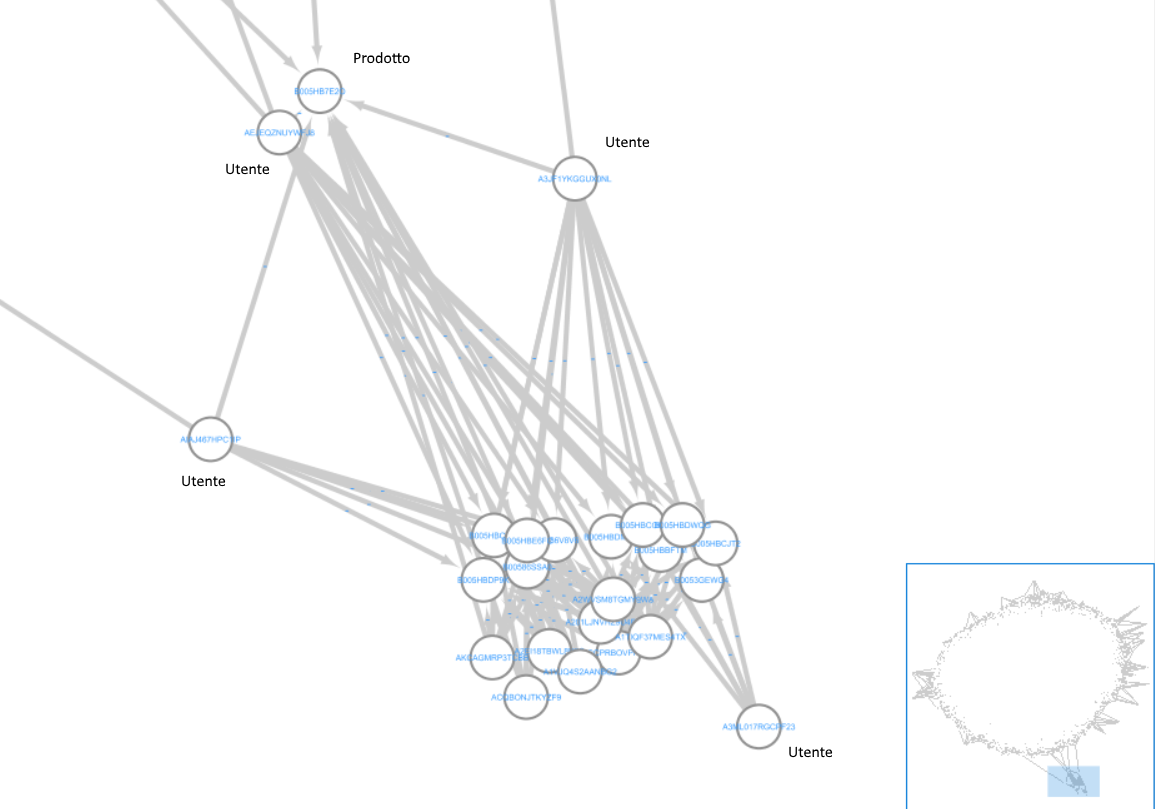
\includegraphics[scale=0.36]{images/03_03_cyto_net_3.png}
	\caption[Cluster inferiore della rete]{Cluster inferiore della rete}
	\label{fig:cyto-net-3}
\end{figure}



\subsection{Grado dei nodi}
\label{sec:nodes-degree}

Il principale motivo per cui si è deciso di costruire la rete associata al dominio in esame è l'analisi del grado dei nodi facenti parte della rete. Per come essa è stata costruita, l'\textit{out-degree} di un nodo rappresenta le recensioni fatte da un utente, mentre l'\textit{in-degree} costituisce quelle ricevute da un prodotto. É chiaro che ogni nodo avrà sempre uno dei due gradi uguale a zero.

Particolarmente rilevante è quindi la distribuzione dei due gradi, al fine di comprendere se all'interno del dataset compaiano utenti e prodotti con un eguale distribuzione di recensioni, piuttosto che invece utenti particolarmente attivi o prodotti molto popolari. Si fa inoltre notare che, come accennato nella sezione \ref{sec:dataset}, il grado minimo di ciascun nodo è pari a cinque poiché il dataset è ottenuto attraverso l'estrazione di un sottografo 5-induttivo da una rete molto più grande.

Osservando in figura \ref{fig:out-degree} ed escludendo dall'analisi i nodi con \textit{out-degree} pari a zero (cioè i prodotti), è possibile notare che nonostante la media di recensioni per utente sia pari a 7 (vedere sezione \ref{sec:dimensions}), in realtà il grado per ciascun nodo è distribuito in maniera piuttosto varia con una frequenza che diminuisce all'aumentare del grado. Solo sei sono gli utenti con più di 60 recensioni, di cui uno ne conta ben 136. Eccoli:

\begin{verbatim}
[('A2J4XMWKR8PPD0', 136),('A2GA55P7WGHJCP', 76),('A2KBV88FL48CFS', 69),
 ('AENH50GW3OKDA', 68),('A2V5R832QCSOMX', 62),('AVUJP7Z6BNT11', 61)]
\end{verbatim}

\begin{figure}[H]
	\centering
	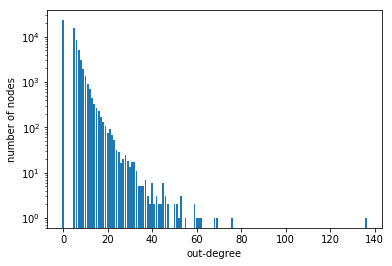
\includegraphics[scale=0.7]{images/03_04_out_degree.png}
	\caption[Distribuzione dell'\textit{out-degree} per gli utenti]{Distribuzione dell'\textit{out-degree} per gli utenti}
	\label{fig:out-degree}
\end{figure}

Anche considerando il grafico della distribuzione degli \textit{in-degree} (figura \ref{fig:in-degree}) si nota che molti prodotti si discostano dalla media di 12 recensioni precedentemente calcolata e addirittura esistono all'interno del dataset prodotti particolarmente popolari con più di 200 recensioni. Sebbene sia un numero elevato, probabilmente non è necessario affinché questi possano definirsi \textit{hub}, vista la presenza nella rete di ben 23.033 prodotti per più di 250.000 recensioni. Di seguito i quattro prodotti più popolari:

\begin{verbatim}
[('B005LERHD8', 441),('B005GYGD7O', 286),('B008WYDP1C', 249),
 ('B0058XIMMM', 241),('B00CKGB85I', 225),('B007RD9DS8', 217)]
\end{verbatim}

\begin{figure}[H]
\centering
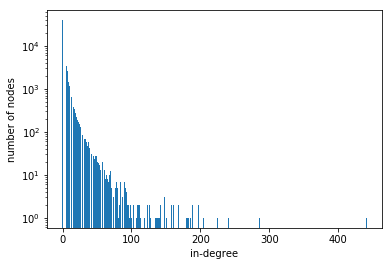
\includegraphics[scale=0.7]{images/03_04_in_degree.png}
\caption[Distribuzione dell'\textit{in-degree} per i prodotti]{Distribuzione dell'\textit{in-degree} per i prodotti}
\label{fig:in-degree}
\end{figure}

\subsection{??? Misure di centralità}



\clearpage



\section{Sentiment Analysis}


La sentiment analysis è il processo che, attraverso l'elaborazione del linguaggio naturale, consente di identificare e estrarre da un testo un'opinione: positiva, negativa o neutrale. Ci sono varie tecniche che è possibile adottare per svolgere sentiment analysis, che ha inizio dal pre-processing del testo al fine di identificare le parole utilizzate e successivamente classificarne il sentiment.

La polarità espressa da ciascuna parola, che successivamente può contribuire all'identificazione di un sentiment per l'intera frase, può essere reperita in un vocabolario linguistico piuttosto che attraverso un dizionario appreso dai dati a disposizione. Quest'ultimo approccio è realizzabile qualora si abbia un elemento nel dataset da usare come target per la classificazione durante l'apprendimento supervisionato dei termini associati a sentimenti positivi o negativi.

In questo capitolo viene presentata solamente l'analisi preliminare effettuata sul testo delle recensioni nel dataset. Tale analisi sarà seguita nei capitoli successivi da due diversi approcci per l'identificazione del sentiment.



\subsection{Assunzioni}

A causa dell'elevato sbilanciamento della variabile target \texttt{rating}, già emerso nel capitolo \ref{sec:rating-distr}, si è considerato che la maggior parte degli algoritmi di apprendimento supervisionato di sentiment analysis avrebbero performato male sul dataset originale e non filtrato. Per questo motivo, in alcune fasi della sentiment analysis si è deciso di mettere in atto delle contromisure per arginare il problema, e a posteriori è possibile dire che tali scelte si sono rivelate corrette per ottenere dei modelli di predizione (capitolo \ref{sec:sentiment-prediction}) con prestazioni migliori.


\subsubsection{Binarizzazione}

La prima scelta effettuata per ribilanciare le classi del target è stata quella di binarizzare l'outcome. Se il \texttt{rating} è espresso nel dataset su un dominio discreto da 1 a 5 (figura \ref{fig:rating-distr-orig}), considerata l'elevata percentuale di recensioni con punteggio 4 o 5 si è pensato di raggruppare quest'ultime in un'unica classe che esprimesse un sentimento positivo; i valori minori o uguali a 3 sono invece stati raggruppati per rappresentare la classe negativa. In funzione del ridotto numero di recensioni negative, si è preferito in questa sede escludere la considerazione di un'eventuale classe per il sentiment neutrale, anche in funzione della difficoltà di classificazione.


\subsubsection{Undersampling}

A seguito della binarizzazione si sono quindi ottenute 221.597 e 57.080 recensioni con sentiment rispettivamente positivo e negativo. Essendo ancora insufficiente per ottenere buoni modelli di machine learning si è quindi proceduto effettuando undersampling della classe di maggioranza, attraverso una funzione che ha portato alla generazione di un dataset con 57.080 recensioni per entrambi i sentiment considerati.



\subsection{Elaborazione del testo}
\label{sec:text-elab}

Affinché qualsiasi operazione di analisi testuale possa essere portata a termine con successo è necessario che i testi considerati vengano sottoposti a una fase di pre-processing davvero fondamentale. Questa si compone di diversi step, alcuni dei quali facoltativi, che hanno l'obiettivo di suddividere il testo in parole e successivamente normalizzarle sulla base di scelte operative o regole linguistiche.

Vengono qui presentate le fasi generiche di elaborazione di un testo e quindi descritte le modalità attraverso le quali sono state implementate. Si consideri che si sta considerando testo scritto in lingua inglese, pertanto non soggetto alla presenza di caratteri che richiedono trattazioni particolari.

La libreria utilizzata per portare a termine queste operazioni è \texttt{NLTK} (Natural Language Toolkit) \cite{site:nltk}, ampiamente utilizzata dalla community.


\subsubsection{Tokenizer}

La prima fase di elaborazione è sempre quella di tokenizzazione, cioè la suddivisione del testo in \textit{token}, solitamente parole. Per questa operazione è possibile sfruttare spazi e segni di interpunzione, ma anche caratteri speciali, numeri o l'alternarsi di lettere maiuscole e minuscole.

Diverse tecniche sono state utilizzate per questo elaborato. \\
In prima fase si è scelto di effettuare un'analisi relativa alle parole più comuni, quindi si è scelto di costruire un tokenizer basato su una espressione regolare personalizzata: \texttt{[\^\textbackslash d\textbackslash W][\textbackslash w\textbackslash']*}. Questa consente di considerare come \textit{token} tutte le parole, ma non i numeri, e soprattutto di preservare eventuali contrazioni tipiche della lingua inglese per i verbi o il genitivo sassone. \\
Per le fasi successive della sentiment analysis si è invece optato per un tokenizer più standard, solitamente fornito di default dalla libreria in uso.


\subsubsection{Normalizer}

Ottenuto l'elenco dei \textit{token} costituenti un testo è necessario che essi vengano normalizzati. In questa fase si possono eseguire diverse operazioni, come ad esempio la rimozione o modifica di alcuni caratteri (se non precedentemente fatto direttamente sul testo), ma soprattutto e molto più frequentemente la conversione a caratteri minuscoli, come nel caso in esame.


\subsubsection{Stopwords}

Prettamente dipendente dalla lingua che si sta considerando, la rimozione delle stopwords consiste nell'eliminazione dall'elenco di \textit{token} delle parole altamente ricorrenti in una lingua: articoli, preposizioni, alcuni aggettivi, ... É importante rimuovere le stopwords poiché non forniscono informazione alcuna e potrebbero anche degradare le performance delle analisi successivamente applicate al testo.

Per ogni lingua è solitamente a disposizione delle diverse librerie una lista di stopwords. Per questo progetto si è scelto di ottenere la lista di stopwords inglesi ma successivamente modificarla per evitare la rimozione di alcune parole che si sono ritenute potenzialmente utili per la valutazione delle recensioni: "not" e "but" sono due esempi particolarmente rilevanti.


\subsubsection{Stemmer}

Anche la fase di stemmer (come la successiva qui presentata) è fortemente dipendente dalla lingua che si sta analizzando, questa volta derivato dalle regole grammaticali che costituiscono la fine delle parole. Si pensi ad esempio ai plurali o i participi in inglese, costituiti con regole ben precise: l'applicazione di uno stemmer riduce queste parole alla propria forma base contraendo le ultime lettere, pratica particolarmente utile per l'identificazione di concetti ricorrenti. Fra quelle fin'ora descritte lo stemming è l'operazione più dispendiosa in termini computazionali, quindi deve essere applicato di volta in volta effettuando una valutazione di costi e benefici.


\subsubsection{Lemmatizer}

Simile allo stemming, la lemmatization è un tipo di elaborazione linguistica ancora più potente. Anziché limitarsi a troncare la fine di alcune parole come fa uno stemmer, il lemmatizer converte ciascuna nel proprio lemma linguistico: i verbi all'infinito, per esempio. Ciò consente di ottenere una lista di \textit{token} in cui parole simili che riguardano lo stesso concetto semantico vengano ricondotte al medesimo lemma. È sicuramente la fase più dispendiosa fra tutte e sia per motivi computazionali che di reperibilità dei dizionari è quella in genere meno utilizzata.


\subsubsection{Un esempio}

A dimostrazione di quanto appena esplicato, sia per chiarificare i concetti presentati che per fornire un esempio di elaborazione applicata al testo per la sezione successiva, viene qui mostrato una frase esemplificativa per dimostrare il pre-processing testuale applicatovi.

\begin{verbatim}
Testo:
"Hi! This... isn't a beautiful sentence with some interesting 
$70 and $5,50 features like people's names and Mr.  Fox thoughts 
for number such as 23, 4 and 7 or peer2peer and wi-fi with 
snake_case but not kebab-case."

Tokenization e lowercasing:
['hi', 'this', "isn't", 'a', 'beautiful', 'sentence', 'with', 
'some', 'interesting', 'and', 'features', 'like', "people's", 
'names', 'and', 'mr', 'fox', 'thoughts', 'for', 'number', 
'such', 'as', 'and', 'or', 'peer2peer', 'and', 'wi', 'fi', 
'with', 'snake_case', 'but', 'not', 'kebab', 'case']

Rimozione stopwords:
['hi', "isn't", 'beautiful', 'sentence', 'interesting', 'features', 
'like', "people's", 'names', 'mr', 'fox', 'thoughts', 'number', 
'peer2peer', 'wi', 'fi', 'snake_case', 'but', 'not', 'kebab', 'case']

Stemming:
['hi', "isn't", 'beauti', 'sentenc', 'interest', 'featur', 'like', 
'peopl', 'name', 'mr', 'fox', 'thought', 'number', 'peer2peer', 
'wi', 'fi', 'snake_cas', 'but', 'not', 'kebab', 'case']
\end{verbatim}



\subsection{Parole più comuni}

A seguito dell'elaborazione testuale apportata sui campi \texttt{text} e \texttt{summary} del dataset, come descritto nella precedente sezione, si sono quindi potute calcolare le parole più ricorrenti all'interno del dataset. Per ottenere questo risultato e soprattutto visualizzarlo in maniera accattivante si è scelto di utilizzare la libreria \texttt{WordCloud} \cite{site:wordcloud}, appositamente pensata per ottenere questo tipo di risultato.

Nelle figure \ref{fig:wordcloud-all}, \ref{fig:wordcloud-pos}, \ref{fig:wordcloud-neg} vengono quindi riportate le parole più comuni all'interno del campo \texttt{text} del dataset, prima considerando tutte le recensioni e successivamente solo quelle positive e negative.

\begin{figure}[H]
	\centering
	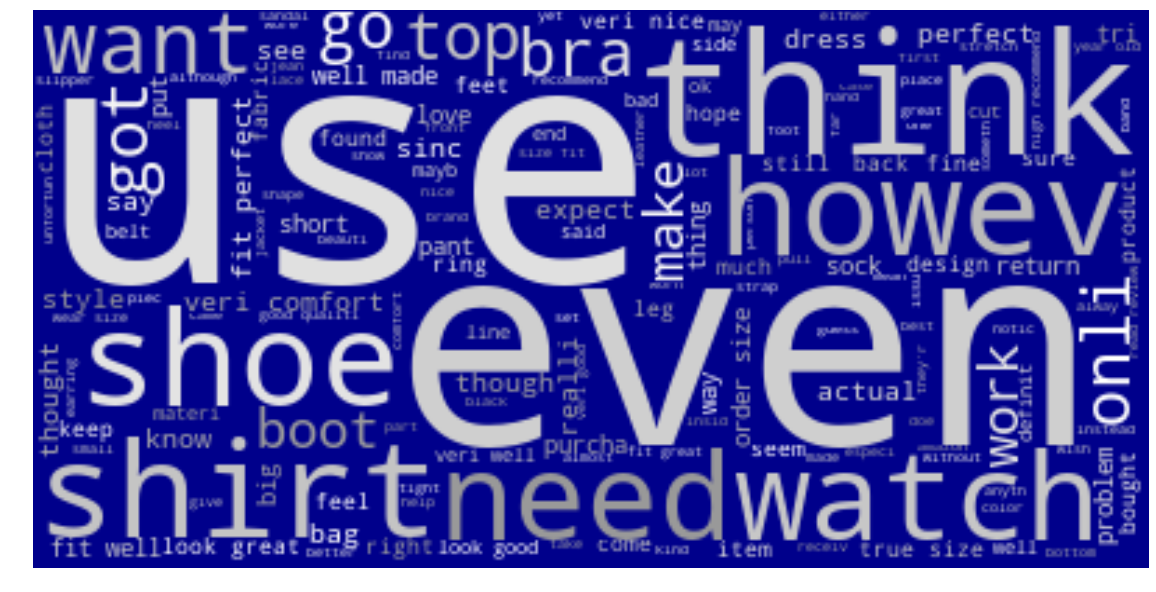
\includegraphics[scale=0.36]{images/04_01_wordcloud_all.png}
	\caption[Parole più comuni in TUTTE le recensioni]{Parole più comuni in TUTTE le recensioni}
	\label{fig:wordcloud-all}
\end{figure}

\begin{figure}[H]
	\centering
	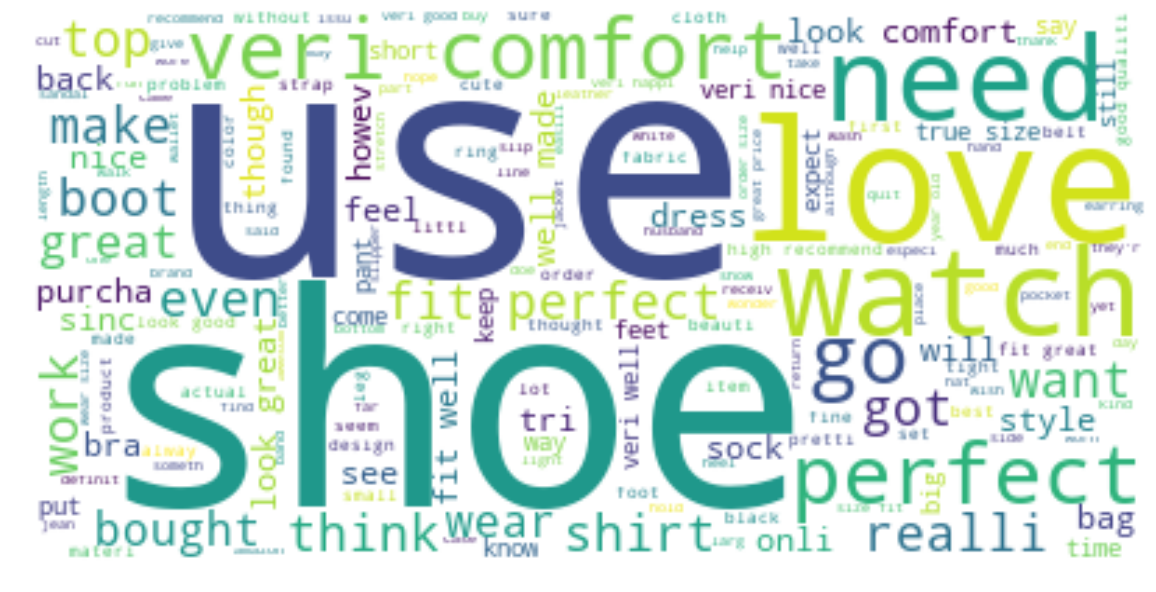
\includegraphics[scale=0.36]{images/04_02_wordcloud_pos.png}
	\caption[Parole più comuni nelle recensioni POSITIVE]{Parole più comuni nelle recensioni POSITIVE}
	\label{fig:wordcloud-pos}
\end{figure}

\begin{figure}[H]
	\centering
	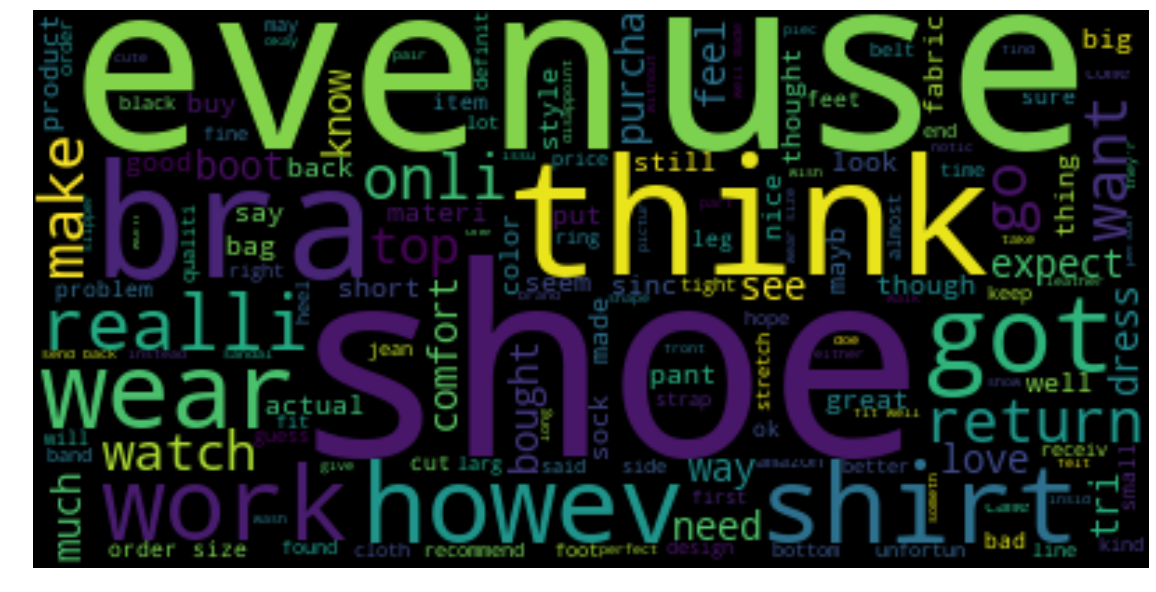
\includegraphics[scale=0.36]{images/04_03_wordcloud_neg.png}
	\caption[Parole più comuni nelle recensioni NEGATIVE]{Parole più comuni nelle recensioni NEGATIVE}
	\label{fig:wordcloud-neg}
\end{figure}


\subsubsection{Alcune considerazioni}

Come si evince dalle WordCloud, è possibile notare che alcune parole siano ricorrenti per entrambi i sentiment. Questo comportamento è del tutto normale per alcune parole tipiche del linguaggio che si sta considerando, utilizzate spesso in tutte le recensioni. Anche quelle negative per esempio potrebbero contenere parole di natura positiva, ma spesso negate attraverso l'utilizzo di avverbi di negazione.

Questo è il motivo per cui molte parole, seppur sembrerebbe logico inserirle nella lista di stopwords affinché non vengano impropriamente considerate, possono comunque rivelarsi utili sia per task di sentiment prediction (capitolo \ref{sec:sentiment-prediction}) che di aspect based sentiment analysis (capitolo \ref{sec:absa}). Questa affermazione è confermata da alcuni test eseguiti proprio inserendo alcune parole comune ad entrambi i sentiment all'interno della lista di stopwords: le performance dei risultati subivano un peggiormento.



\clearpage



\section{Sentiment Prediction}
\label{sec:sentiment-prediction}


Quando si ha a che fare con un dataset di testi su cui si vuole fare sentiment analysis, uno degli aspetti più interessanti è la possibilità di predire il sentiment di nuove recensioni attraverso l'analisi del linguaggio naturale. Ciò è possibile attraverso la classificazione delle parole utilizzate in sentiment positivo e negativo; tale operazione può essere eseguita attraverso l'utilizzo di un vocabolario linguistico, oppure tramite apprendimento di un dizionario dal testo purché il dataset metta a disposizione una variabile target su cui fare apprendimento supervisionato.

Quest'ultimo caso rappresenta perfettamente la situazione che si sta tentando di analizzare, ed è per questo che si è scelto di verificare se un algoritmo di Machine Learning di apprendimento supervisionato sia in grado di ottenere buoni risultati in termini di analisi del linguaggio naturale.

In questo capitolo vengono quindi descritte le fasi generiche necessarie ad effettuare supervised sentiment prediction, implementate poi attraverso l'utilizzo della libreria \texttt{scikit-learn} \cite{site:sklearn}, facilmente utilizzabile e ampiamente diffusa per la fruizione di svariati modelli di Machine Learning.



\subsection{Bag of words}


In ogni occasione in cui si lavora con il testo, che sia essa per apprendimento o anche semplicemente per effettuare una ricerca, è necessario che questo venga memorizzato in una modalità che lo renda facilmente rappresentabile e recuperabile.

Uno dei modelli più utilizzati per ottenere questo obiettivo è il cosiddetto bag of words, implementato da \texttt{scikit-learn} attraverso la classe \texttt{CountVectorizer}. Ciò consiste nella rappresentazione del testo in parole, ad ognuna delle quali viene associato un identificativo; successivamente, di ciascuna parola viene salvata la lista di \textbf{occorrenze} nei documenti che costituiscono il dataset (i record, ad esempio). Così facendo è possibile ottenere di fatto una matrice molto grande e di natura sparsa, contenente le informazioni necessarie a rappresentare il testo per parole, d'ora in poi chiamate più correttamente \textbf{termini}.


\pagebreak


\subsection{Pesatura dei termini (TF-IDF)}

Suddividendo il testo originale in quello che è stata definita bag of words, si ottiene di fatto un \textbf{dizionario} rappresentativo della base di dati testuale. Nonostante sia stato precedentemente detto che per ogni termine si memorizzino le occorrenze nei documenti del dataset, sarebbe più corretto dire che di questi dovrebbero essere salvate le \textbf{frequenze}, opportunamente normalizzate, che rappresentano una più accurata modalità di rappresentazione dell'importanza di ciascuna parola nel testo.

Un modello molto famoso e utilizzato oggi, specialmente nell'ambito dell'Information Retrieval, è conosciuto con il nome di \textbf{TF-IDF (term frequency - inverse document frequency)}. Tale statistica è in grado di computare l'importanza di un termine per ciascun documento presente in un corpus (collezione di testi), sia facendo riferimento alle occorrenze nel documento stesso che alla popolarità della parola nell'intera collezione. Il peso di un termine $i$ nel documento $j$ si esprime con la formula sottostante, in cui il primo fattore del prodotto è la TF (normalizzata) e il secondo invece la IDF ($N$ è il numero di documenti, mentre \(d_{fi}\) rappresenta il numero di documenti che contengono il termine considerato).

\[ w_{ij} = \frac{tf_{i}}{\max tf_{j}} \times log\frac{N}{d_{fi}} \]

Il concetto di TF-IDF è facilmente utilizzabile da \texttt{scikit-learn} attraverso la classe \texttt{TfidfTransformer} per ricavare dalla semplice bag of words una matrice computata secondo TF-IDF. Questo è successivamente utilizzato da un modello di classificazione a piacere per effettuare l'apprendimento supervisionato.

La libreria permette inoltre di accorpare le funzionalità di \texttt{CountVectorizer} e \texttt{TfidfTransformer} nell'utilizzo di un'unica classe: \texttt{TfidfVectorizer}. Tale classe è inoltre in grado di effettuare la pre-elaborazione del testo esplicata nel capitolo \ref{sec:text-elab}, previa configurazione con appositi parametri dall'utilizzo estremamente facile. 

\vspace{6ex}

\subsubsection{Termini più rilevanti}

Applicando i concetti appena descritti al dataset in esame si ottiene il peso di ciascun termine presente nel testo delle recensioni. Per completezza è interessante notare quali sono i termini che TF-IDF considera più rilevanti dopo la computazione del dizionario. Questi sono mostrati nella tabella \ref{tab:term-weights}

\begin{table}[H]
	\caption{Termini più rilevanti secondo TF-IDF}\label{tab:term-weights}
	\centering
	\begin{tabular}{|l|l|l|}
		\hline
		ID & Termine & Peso \\
		\hline
		4121 & but & 0.040886 \\ 
		19248 & not & 0.037178 \\ 
		25748 & size & 0.033456 \\ 
		31509 & veri & 0.032994 \\ 
		10467 & fit & 0.032224 \\ 
		16499 & look & 0.030117 \\ 
		16151 & like & 0.029839 \\ 
		32213 & wear & 0.029403 \\ 
		25314 & shoe & 0.027903 \\ 
		16656 & love & 0.025427 \\ 
		\hline
	\end{tabular}
\end{table}



\subsection{Modelli di predizione}

Appreso il dizionario del testo, è possibile utilizzarlo come input di un classificatore insieme alla colonna del target per apprendere il modello di Machine Learning. Lo scopo è trovare una correlazione fra il testo di una recensione e il suo sentiment. \\
É possibile utilizzare lo stesso dizionario per svariati modelli, ampiamente configurabili. Ai fini dell'esperimento ne sono stati provati tre: Random Forest, Naive Bayes e SVM. Vengono quindi presentate le performance ottenute da ciascuno, considerando una separazione fra training e test set del 70-30\% con rimescolamento.

Verranno riportate per ciascun modello tutte le metriche valutate. Mentre la matrice di confusione, così come ROC e AUROC sono ottenute da una singola esecuzione, le metriche di accuracy, recall, precision e F1 sono invece ricavate attraverso l'esecuzione di una 10-fold cross validation.


\subsubsection{Random Forest}

Random Forest è dei tre il modello con le peggiori performance, qui riportate. Bisongna considerare che rispetto agli altri modelli è anche decisamente più lento nell'apprendimento (nell'ordine di un paio di minuti, contro una decina di secondi per NB e SVM).

\begin{verbatim}
RandomForestClassifier(
   bootstrap=True, class_weight=None, criterion='gini',
   max_depth=None, max_features='auto', max_leaf_nodes=None,
   min_impurity_decrease=0.0, min_impurity_split=None,
   min_samples_leaf=1, min_samples_split=2,
   min_weight_fraction_leaf=0.0, n_estimators=5, warm_start=False)
\end{verbatim}

\begin{figure}[H]
	\centering
	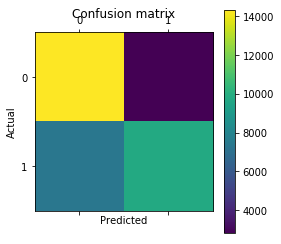
\includegraphics[scale=0.6]{images/05_00_rf_confmat.png}
	\caption[Random Forest - Matrice di confusione]{Random Forest - Matrice di confusione}
	\label{fig:rf-cm}
\end{figure}

\begin{figure}[H]
\centering
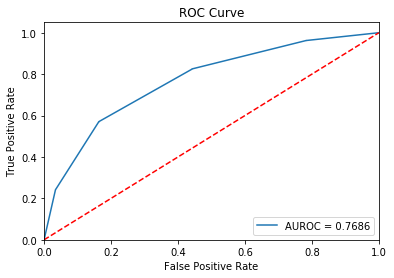
\includegraphics[scale=0.6]{images/05_00_rf_auroc.png}
\caption[Random Forest - ROC e AUC]{Random Forest - ROC e AUC}
\label{fig:rf-auroc}
\end{figure}

\begin{verbatim}
ACCURACY    10-FOLD CROSS VALIDATION:    0.7327 (std dev 0.005981)
PRECISION   10-FOLD CROSS VALIDATION:    0.7348 (std dev 0.009141)
RECALL      10-FOLD CROSS VALIDATION:    0.7348 (std dev 0.008359)
F1          10-FOLD CROSS VALIDATION:    0.7279 (std dev 0.003274)
\end{verbatim}

\clearpage

\subsubsection{Naive Bayes}

\begin{verbatim}
MultinomialNB(alpha=1.0, class_prior=None, fit_prior=True)
\end{verbatim}

\begin{figure}[H]
	\centering
	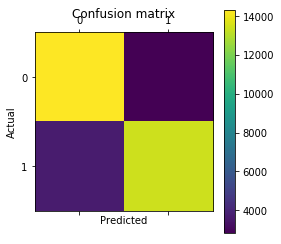
\includegraphics[scale=0.6]{images/05_01_bayes_confmat.png}
	\caption[Naive Bayes - Matrice di confusione]{Naive Bayes - Matrice di confusione}
	\label{fig:bayes-cm}
\end{figure}

\begin{figure}[H]
	\centering
	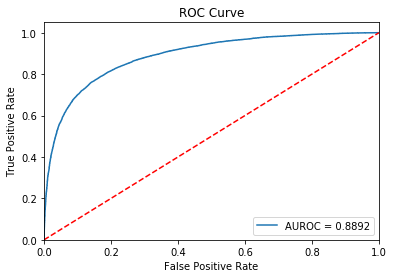
\includegraphics[scale=0.6]{images/05_01_bayes_auroc.png}
	\caption[Naive Bayes - ROC e AUC]{Naive Bayes - ROC e AUC}
	\label{fig:bayes-auroc}
\end{figure}

\begin{verbatim}
ACCURACY    10-FOLD CROSS VALIDATION:    0.8015 (std dev 0.007751)
PRECISION   10-FOLD CROSS VALIDATION:    0.8116 (std dev 0.014807)
RECALL      10-FOLD CROSS VALIDATION:    0.7858 (std dev 0.007262)
F1          10-FOLD CROSS VALIDATION:    0.7984 (std dev 0.006062)
\end{verbatim}

\clearpage

\subsubsection{Support Vector Machines}

\begin{verbatim}
SGDClassifier(
   alpha=0.0001, average=False, class_weight=None,
   early_stopping=False, epsilon=0.1, eta0=0.0, fit_intercept=True,
   l1_ratio=0.15, learning_rate='optimal', loss='log', max_iter=1000,
   n_iter_no_change=5, n_jobs=None, penalty='l2', power_t=0.5,
   random_state=None, shuffle=True, tol=0.001,
   validation_fraction=0.1, verbose=0, warm_start=False)
\end{verbatim}

\begin{figure}[H]
	\centering
	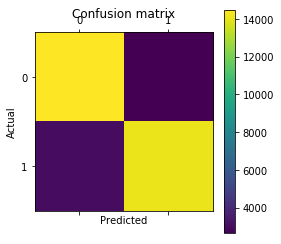
\includegraphics[scale=0.6]{images/05_02_svm_confmat.png}
	\caption[SVM - Matrice di confusione]{SVM - Matrice di confusione}
	\label{fig:svm-cm}
\end{figure}

\begin{figure}[H]
	\centering
	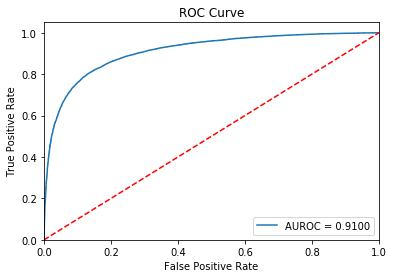
\includegraphics[scale=0.6]{images/05_02_svm_auroc.png}
	\caption[SVM - ROC e AUC]{SVM - ROC e AUC}
	\label{fig:svm-auroc}
\end{figure}

\begin{verbatim}
ACCURACY    10-FOLD CROSS VALIDATION:    0.8290 (std dev 0.005217)
PRECISION   10-FOLD CROSS VALIDATION:    0.8371 (std dev 0.009706)
RECALL      10-FOLD CROSS VALIDATION:    0.8176 (std dev 0.008412)
F1          10-FOLD CROSS VALIDATION:    0.8273 (std dev 0.004608)
\end{verbatim}


\subsubsection{Scelta del modello}

Come mostrato, Naive Bayes e SVM ottengono performance molto simili. Il primo è più rapido nell'apprendimento, ma il secondo ottiene un paio di punti percentuali in più su tutte le metriche. Per questo motivo, si è scelto di utilizzare SVM per le predizioni future.



\subsection{Pipeline}

Scelta la modalità di elaborazione del testo e il classificatore più adeguato per il dominio di riferimento, \texttt{scikit-learn} consente di effettuare predizioni sui nuovi input. Chiaramente non è necessario che vengano effettuate ogni volta le operazioni preliminari di apprendimento sull'intero dataset, ma è sufficiente sfruttare il modello appreso a cui fornire il nuovo input, adeguatamente pre-processato. Per agevolare il processo, la classe \texttt{Pipeline} fornisce al programmatore la possibilità di definire una sequenza di operazioni necessaria sia per l'apprendimento che per la predizione su nuovi input.

É sufficiente quindi salvare il modello su un file persistente per poterlo riutilizzare successivamente. Questa è anche la tecnica adottata per il funzionamento della Web demo che verrà presentata nel capitolo \ref{sec:ui}. Per completezza, si riporta qui anche il codice della pipeline scelta per effettuare i nostri task di sentiment prediction.

\begin{verbatim}
text_clf = Pipeline([
     ('vect', TfidfVectorizer(
                  use_idf = True,
                  strip_accents = 'ascii',
                  stop_words = stopset,
                  lowercase = True)),
     ('tfidf', TfidfTransformer()),
     ('clf', SGDClassifier(loss='log')),
])
\end{verbatim}



\clearpage



\section{Aspect Based Sentiment Analysis}
\label{sec:absa}


Se nel capitolo precedente è stata presentata una forma di sentiment analysis basata su un modello di apprendimento supervisionato, non è sempre ovvio che nel dataset da analizzare sia presente il target su cui effettuare la classificazione. Inoltre, l'avanzamento della ricerca nell'ambito del Natural Language Processing (NLP) ha permesso ai ricercatori di addestrare svariati modelli negli anni e quindi apprendere e pubblicare dei vocabolari standard che permettono, sia attraverso un'analisi morfologica che semantica, di valutare il sentiment di un insieme di parole.

In questo contesto nasce l'aspect based sentiment analysis (ABSA) il cui scopo è l'estrazione degli \textbf{aspetti} da una base testuale, cioè dei concetti descritti al suo interno, e la loro conseguente classificazione come positivamente o negativamente valutati dal testo attraverso l'utilizzo di vocabolari consolidati nel tempo. Ciò consente a chi analizza un corpus di ottenere una visione d'insieme non solo relativa all'opinione generica dei propri utenti, ma anche riguardo specifici aspetti (caratteristiche del prodotto, ad esempio). Questo permette alle aziende di migliorare ulteriormente il proprio servizio e porsi ovviamente su una più alta fascia di mercato.



\subsection{Strumenti}

L'aspect based sentiment analysis è un argomento meno approfondito allo stato dell'arte attuale rispetto agli argomenti precedenti trattati. Sebbene esistano numerosi articoli che ne parlano e anche alcuni servizi a pagamento che consentono di fare ABSA, è molto più complicato - se non impossibile - trovare delle librerie open source che permettano di eseguire rapidamente l'intera pipeline necessaria a questo tipo di analisi, come invece è possibile fare per il sentiment prediction supervisionato.

In funzione di queste considerazioni, si è deciso di valutare l'opportunità di riprendere un progetto open source scritto in Python e già avviato su GitHub, per ri-adattarlo alle esigenze di questo studio \cite{site:jonm01-absa}. Dopo qualche esperimento, l'utilizzo di tale progetto si è rivelato la scelta adatta a soddisfare i requisiti richiesti per implementare correttamente aspect based sentiment analysis.



\subsection{Elaborazione del testo}

Nonostante sia stato accennato che questa tecnica di analisi sia fondamentalmente diversa dalla precedente, bisogna notare che la trattazione preliminare dei testi avviene in modo totalmente analogo. I principi spiegati nel capitolo \ref{sec:text-elab} rimangono validi e devono solamente essere riadattati per adeguarsi alle successive fasi di analisi.

Nello specifico, le operazioni che si è scelto di effettuare sull'input sono le seguenti:

\begin{itemize}
	\item rimozione stop word
	\item suddivisione in frasi
	\item rimozione delle domande: poco significative o sarcastiche
	\item POS tagging (approfondito nella sezione successiva)
	\item lemmatization, con il supporto del precedente POS tagging
\end{itemize}


\subsubsection{POS tagging}

Acronimo di \textit{part-of-speech tagging}, consiste nell'assegnazione di un tag per ciascuna parola del testo, al fine di identificare la categoria grammaticale a cui appartiene. Linguisticamente parlando, il termine \textbf{parte del discorso} definisce le categorie di parole atte a formare le frasi di una lingua, definite dalla disciplina chiamata \textbf{morfologia}. Nella lingua inglese sono distinte in: nomi, aggettivi, verbi, proposizioni, avverbi, pronomi, congiunzioni e interiezioni.

Il processo di POS tagging, quindi, analizza una frase e si occupa di assegnare il ruolo di nome, aggettivo, verbo, etc. ad ogni parola che la compone. Tale operazione è svolta nel codice attraverso l'utilizzo della funzione \texttt{pos\_tag} della libreria \texttt{NLTK}, precedentemente utilizzata anche per le altre fasi dell'elaborazione testuale.



\subsection{Estrazione degli aspetti}



\subsection{Identificazione del sentiment}



\subsection{Risultati}




\clearpage



\section{Collaborative Filtering}

\subsection{Funzionamento}

\subsection{Risultati}



\clearpage



\section{Web Demo}
\label{sec:ui}


\subsection{Architettura}

L'interfaccia web è stata sviluppata utilizzando l'architettura a 3 layer, con separazione di frontend, backend e database.

Il database utilizzato in fase di lettura è quello fornito inizialmente, senza alcuna modifica. Esso consiste quindi in un file SQLite interrogabile e modificabile semplicemente tramite un web server. Questo risulta particolarmente utile per fornire i dettagli dei giocatori ed eventualmente dei team così che l'utente possa visualizzarli e sceglierli attraverso l'opportuna interfaccia.

Per lo sviluppo del backend è stato deciso di utilizzare l'engine Javascript tramite il popolare progetto Node.js \cite{site:nodejs}. Esso è in grado di agire come middleware tra il frontend e il database, separando al meglio le logiche di manipolazione del dato. \'E inoltre incaricato di chiamare adeguatamente lo script R per la predizione del vincitore della partita e per svolgere le inferenze richieste.

Il frontend è invece sviluppato utilizzando la libreria Javascript React.js \cite{site:react}



\subsection{Sentiment Prediction}

\subsection{Aspect Based Sentiment Analysis}



\clearpage



\section{Conclusioni}

Lo studio è riuscito a dimostrare le innumerevoli possibilità di effettuare analisi sul dominio delle recensioni. Considerando sia l'elaborazione del linguaggio naturale che l'analisi sulla rete è possibile ottenere risultati molto importanti e anche piuttosto precisi sotto diversi aspetti, che possono sicuramente rappresentare un contributo fondamentale al miglioramento del business di un'azienda.

In particolare, analizzare le recensioni di Amazon può essere utile sia ai venditori che al portale di e-commerce stesso per migliorare i propri servizi o sapere come ampliare l'offerta commerciale, curando magari gli aspetti più carenti. Con assoluta certezza si potrebbe appurare che parte del successo di Amazon è stato acquisito anche grazie ad analisi di questo tipo.

I medesimi modelli possono essere facilmente riadattati a qualsiasi altro dominio preveda l'utilizzo di recensioni e sarebbe sicuramente curioso sapere quali dei principali colossi tech odierni abbiano sfruttato metodologie di sentiment analysis per scalare le vette di mercato. Allo stesso modo, uno sviluppo futuro potrebbe essere rappresentato dalla possibilità di comprendere se i metodi presentati sono ugualmente performanti anche sull'analisi dei commenti di un social network, per esempio.




\newpage
\bibliographystyle{plainurl}
\bibliography{biblist}
	
\end{document}
